%======================================================================
\subsection{BW-ROU-01..04 --- Built, 27 Oct: route paths, wires, pipes, hoses, the BOM by length}\label{sec:rou-built}
%======================================================================

The track above was built the same evening, in five commits (\code{8c658f96} ROU-01, \code{2c4081cf} ROU-02,
\code{8b4b8bb3} ROU-03, \code{bf8a16d0} ROU-04, plus the wire default below), all Python: the maths FreeCAD-free in
\file{addons/BruceWorx/bruceworx/routing.py}, the objects in \file{src/Mod/BruceWorx/bruceworx\_routing.py}, the
commands and panels in \file{bruceworx\_routing\_gui.py}, nine icons, and a Routing tab in the Design workspace
(\file{workspaces.json}: Path $\cdot$ Items $\cdot$ Reports). Your decisions were kept: our own Routing workspace,
not the Cables add-on; \code{Part::FeaturePython} objects that share Keystone's panels, the part-properties schema
and the vault BOM.

\begin{figure}[!htbp]
\centering
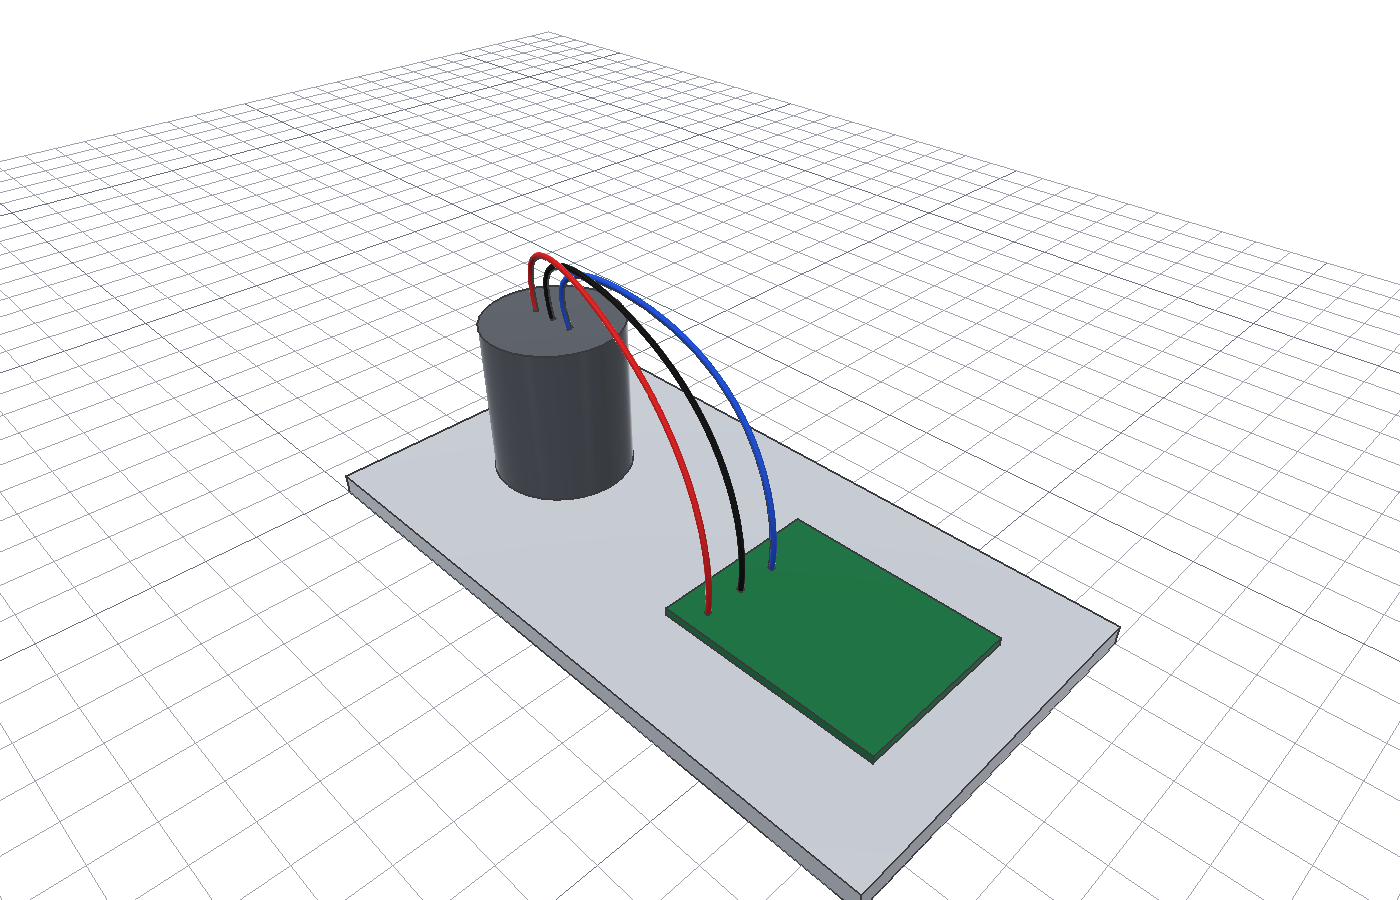
\includegraphics[width=0.49\linewidth]{fig/routing_harness.png}\hfill
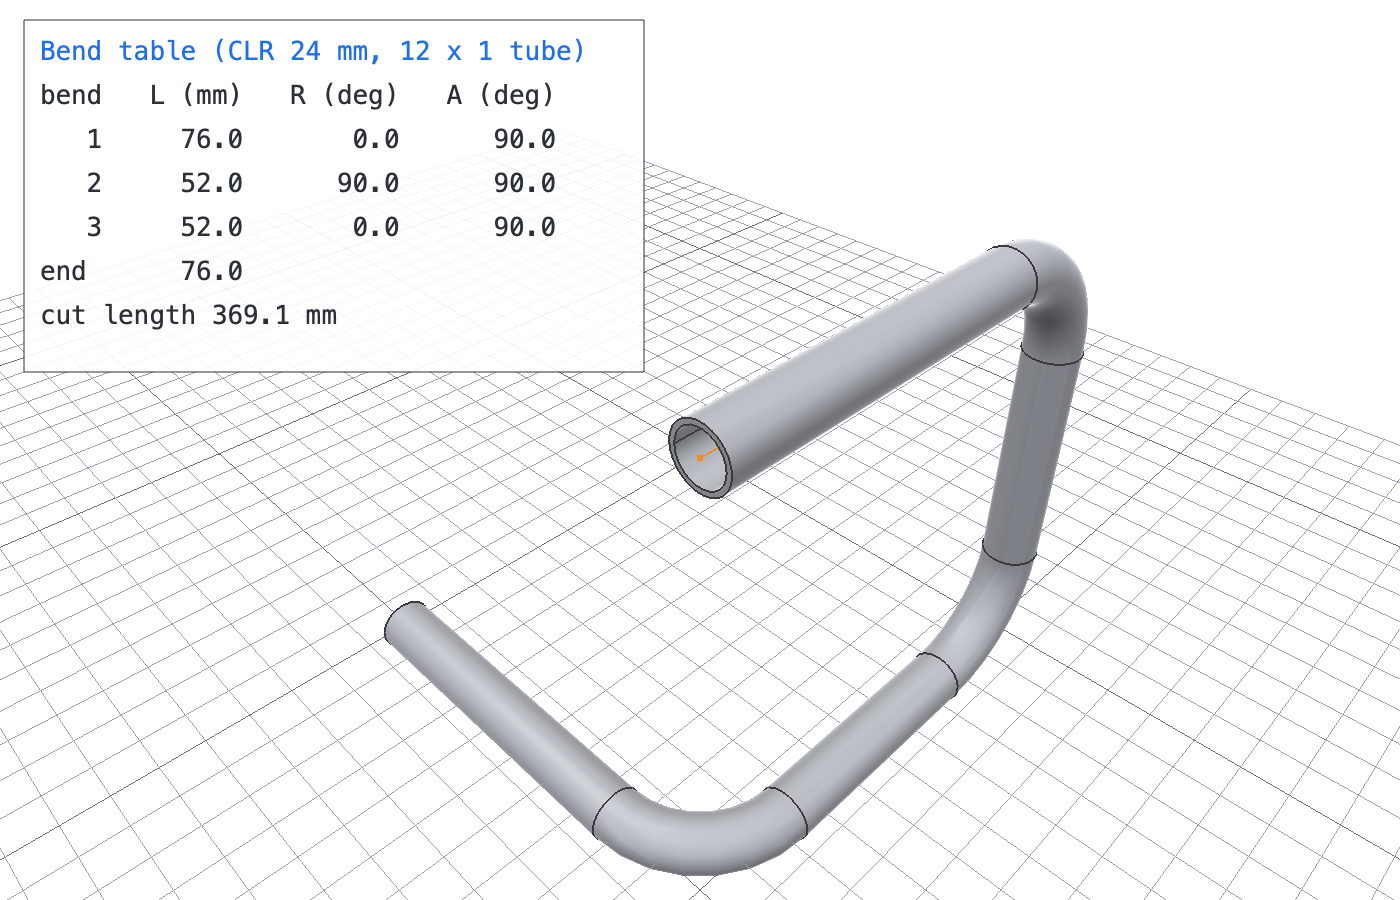
\includegraphics[width=0.49\linewidth]{fig/routing_tube.png}
\caption{Left: a motor-to-board harness, three 22\,AWG wires (+12V red, GND black, HALL blue) on three spline
paths from the motor's terminals to the board's pads; the from-to list reads 0.100, 0.093 and 0.088\,m with 5\,\%
slack, 0.39, 0.36 and 0.34\,g. Right: a 12\,$\times$\,1 tube on a four-corner polyline path at the default CLR of
24\,mm with its bend table and cut length (369.1\,mm $= 4\times$ straights $76+52+52+76$ plus three quarter arcs of
$24\pi/2$). Both are off-screen renders of the real objects.}
\label{fig:routing-built}
\end{figure}

\paragraph{What you can do now.}
\begin{itemize}[nosep]
  \item \textbf{Route Path} (the panel in Fig.~\ref{fig:routing-mock}): click vertices, circular edges (their centre),
        faces (their centre) or datums and LCS (their origin) in the 3D view; each pick is a point of the path and
        is \emph{attached} to what was picked, so moving the motor re-routes the wire (checked: a box moved 30\,mm
        along X and 60 along Y takes its vertex and the path's end with it). The list can be reordered and
        trimmed; mode (Spline or Polyline with arcs), bend radius and minimum bend radius are live; the panel shows
        the length, the bend count, the tightest radius and the check, in red when a corner does not fit or a bend
        is below the minimum. Cancel undoes everything; an existing path opens in the same panel. \textbf{Add
        Point} appends the selection to the open panel or to the selected path; \textbf{Clip} attaches the nearest
        point of the selected path to the picked geometry.
  \item \textbf{Wire, Pipe, Hose}: one short form each on the selected path (or the document's only one), live on
        the object: gauge (30\,AWG to 0\,AWG and 0.25--10\,mm$^2$), insulation OD (from the gauge when left at
        zero), colour (a colour dialog; the 3D view follows), signal, from/to connector and pin, slack; tube size
        (metric OD\,$\times$\,wall and NPS schedule 40, or Custom), wall, material, CLR, minimum radius; hose ID,
        OD, minimum radius, slack. The panel prints the length in mm and m, a wire's mass, a pipe's cut length and
        bend table, and the too-tight warning. \textbf{Bundle} groups the selected wires (combined OD
        $1.15\sqrt{\sum\text{OD}_k^2}$, drawn translucent).
  \item \textbf{From-to list} and \textbf{Cut list}: CSV files written where the file dialog says (wire, signal,
        gauge, colour, from, from pin, to, to pin, length in m; item, kind, size, cut length, bend radius, bends,
        the LRA rows as text).
  \item \textbf{The Browser} shows a ``bend too tight'' badge on any path, wire, pipe or hose whose \code{BendOK}
        is false; the object's \code{Problems} property says why.
  \item \textbf{The BOM.} Every routed item carries \code{QuantityUnit} = m and \code{QuantityPer} = its length in
        metres, two new properties in the lowest layer of the part-properties schema (every part gets them, 1 and
        empty for a counted part). The vault's BOM walker lists a wire, pipe or hose by length (``1.25\,m'' in
        the Qty and Total cells of the indented and flattened BOM and their CSVs, metered lines may be fractional,
        counts stay whole) and skips the RoutePath itself. The Assembly BOM needed no C++: its Quantity column
        counts occurrences and the \code{.QuantityUnit} / \code{.QuantityPer} property columns give the length.
\end{itemize}

\paragraph{Decided while building.}
\begin{itemize}[nosep]
  \item \textbf{Two splines, one truth.} The FreeCAD shape is OCC's interpolation (\code{BSplineCurve.interpolate});
        the object measures \emph{that} curve (\code{Edge.curvatureAt} at 120 samples per edge) for the tightest
        radius and its exact length, so the check is on what is drawn. The FreeCAD-free module uses a C2 cubic spline
        with not-a-knot ends and chord-length parameters (analytic $\mathbf r'$, $\mathbf r''$, Simpson length), which
        is what the unit tests and a preview need: 13 points on a semicircle of $R=100$ give the length within
        $10^{-5}$ and the tightest radius 95.7; the OCC curve through 9 points on $R=50$ gives 44.9 (the natural-end
        spline first tried gave 78 of 100 and was dropped). The plan's centripetal parametrisation was not needed
        on route-like point sets.
  \item \textbf{Points live in the document frame; the wire is built in the container frame.} A shape's own
        Placement is overwritten by the object's while it recomputes (\code{Part::Feature::onChanged}), so the
        points are transformed before the wire is made rather than placing the shape afterwards. Items sit in
        their path's container, so a harness inside a placed \code{App::Part} draws where it should.
  \item \textbf{Attachments as triples.} A \code{PropertyLinkSubList} groups its entries by object and loses the
        order, so the path keeps the links there (for the dependency) and the \code{index|object|sub} triples in
        \code{AttachedTo} for the mapping. Found by the GUI test that picks two vertices of one box.
  \item \textbf{A clip is an attachment}, not an object (your R3 recommendation): the Clip command attaches the
        nearest path point to the picked geometry.
  \item \textbf{The pipe's CLR drives its path} in Polyline mode (\code{sync\_clr}): one radius serves the geometry,
        the cut length and the LRA table; a hose on the same path is then checked against it. Defaults: tube CLR
        $2\,$OD, tube minimum $1.5\,$OD, hose $6\,$OD, wire $4\,$OD (R2); the wire default flags the sample harness's
        third wire (tightest 4.0 vs 4.6\,mm), which is the honest answer for a hook-up wire bent that hard.
  \item \textbf{The tube is two pipe shells cut}, as ArchPipe does (outer minus bore), with round transitions; the
        volume of the three-bend tube matches annulus $\times$ cut length within 3\,\%.
  \item \textbf{Colour names.} The from-to list names red, black, white, blue, green and yellow and prints the hex
        value for anything else.
  \item \textbf{Fittings and the menu} were left out (the brief allowed it): no end fittings on pipes, no Vector Labs
        menu entries; the Routing tab is the way in.
\end{itemize}

\paragraph{Tests.} Unit (\file{addons/BruceWorx/tests/test\_routing.py}, 21, in the 538 of the addon suite): a two-point
spline is a line, collinear points stay straight, semicircle length and radius, $\kappa=1/R$ for a circle, the
right-angle route with one arc ($160+10\pi$), overlapping tangents reported (R\,120 on 100\,mm legs; two corners on a
30\,mm middle leg), the three-bend LRA table $(80,0,90),(60,90,90),(60,0,90)$, end 80, the rotation sign, the
summary checks, AWG 22/10/0 and 36, the wire mass, the bundle OD, the tube sizes, both CSVs. Two more in
\file{test\_bom.py}: metered rows summed in metres, a vault BOM with a 1.25\,m line and a 0.4\,m gap, flattened
2.5\,m, a fractional count refused. Headless (\file{TestBruceWorxRoutingCore.py}, 12): a spline path through four
points (length within 1\,\% of the module's spline), the polyline path ($160+10\pi$ exact, bend table, below the
minimum, a radius that does not fit), the spline radius check, attached points that follow a moved box and a
cylinder's circle centre, several attachments on one object out of order, a wire with 5 and 10\,\% slack and its
mass, the pipe's cut length $280+30\pi$ and LRA rows by hand, a hose at $6\,$OD flagged then cleared, the bundle OD,
both reports, save and reload, items in a placed part, the BOM walker on an assembly with a hose and a bolt. GUI
(\file{TestBruceWorxRouting.py}, 7, under \file{run\_gui\_tests.py}): the tab and the nine commands, a path from
picks arriving through the selection observer (face centre, two vertices), reorder, remove, re-add, OK, the moved
part, undo; Cancel removes a new path and the edit panel keeps one; Add Point and Clip; the Wire panel and the
from-to CSV; the Pipe panel (size 16\,$\times$\,1.5, CLR 32), the Hose panel's warning and its Cancel, the Browser
badge and the cut list; the Bundle command. The workspace (25) and connection-lint (15) suites pass with the new
tab.

\paragraph{Open questions for you.}
\begin{enumerate}[nosep]
  \item \textbf{Wire minimum $4\,$OD} flags the sample harness (tightest 4.0 vs 4.6\,mm on 22\,AWG). Keep the rule, or
        $3\,$OD as for silicone tubing?
  \item \textbf{A purchasing BOM per gauge and colour} (your R4) is not there: wires in the assembly file are ``not a
        vault item'' lines by label. Make the harness its own vault item first (R5), then sum per gauge and colour in
        the flattened BOM?
  \item \textbf{The Assembly BOM} shows a wire as Quantity 1 with \code{.QuantityPer} 0.100 in two property columns,
        and lists the RoutePath as a line unless ``only parts'' is set. Add a C++ ``Length'' column
        (Quantity $\times$ QuantityPer with the unit) and skip paths, or leave the spreadsheet as it is?
  \item \textbf{Picks stay selected} while the Route Path panel is open (the selection grows with every click).
        Clear the selection after each pick, as Fusion's point tools do?
  \item \textbf{One spline or two?} The Part shape is OCC's interpolation and bends tighter near the ends than the
        module's not-a-knot spline (90 vs 96 of 100 on a 9-point circle). Build the shape from the module's own
        spline (one source of truth, slightly rounder ends), or keep OCC's?
\end{enumerate}
